\section{Introduction}
%=====================

Let ${\mathcal C} = \{C_1, C_2, \ldots, C_n\}$ be a set of curves.
We wish to compute all \ccHtmlNoLinksFrom{intersection} points between
two curves in the set in an output-sensitive manner, without having to
go over all $O(n^2)$ curve pairs. To this end, we sweep an imaginary line $l$
from $x = -\infty$ to $x = \infty$ over the plane. While sweeping
the plane, we keep track of the order of curves intersecting it.
This order changes at a finite number of \emph{event points}, such that
we only have to calculate the \ccHtmlNoLinksFrom{intersection} points
between two curves when they become contiguous. For more details on the
\emph{sweep-line algorithm} see, for example,~\cite[Chapter~2]{bkos-cgaa-00}.

This chapter describes two functions implemented using the sweep-line
algorithm: computing all \ccHtmlNoLinksFrom{intersection} points among a
given collection of curves, and computing the set of subcurves that are
pairwise interior-disjoint induced by such an input set of curves.

The implementation is robust. It supports general
curves and handles all degenerate cases, including overlapping curves,
vertical segments, and tangency between curves. The robustness of the
algorithm is guaranteed if the functions are instantiated with a traits
class that employs certified computations. This traits class must be a model
of the \ccc{ArrangementTraits_2} concept --- see the
Chapter~\ref{chapterArrangement_2} for more details.

The complexity of the sweep-line algorithm is $O((n + k)\log{n})$ where $n$
is the  number of the input curves and $k$ is the number of
\ccHtmlNoLinksFrom{intersection} points induced by these curves.

\subsection{A Simple Program}
The simple program listed below computes all sub segments induced by 
a set of four input segments illustrated in figure \ref{SL_sec:simple}.
The endpoints of the resulting sub segments are printed out.

\begin{figure}[hbp]
\begin{ccTexOnly}
\centerline{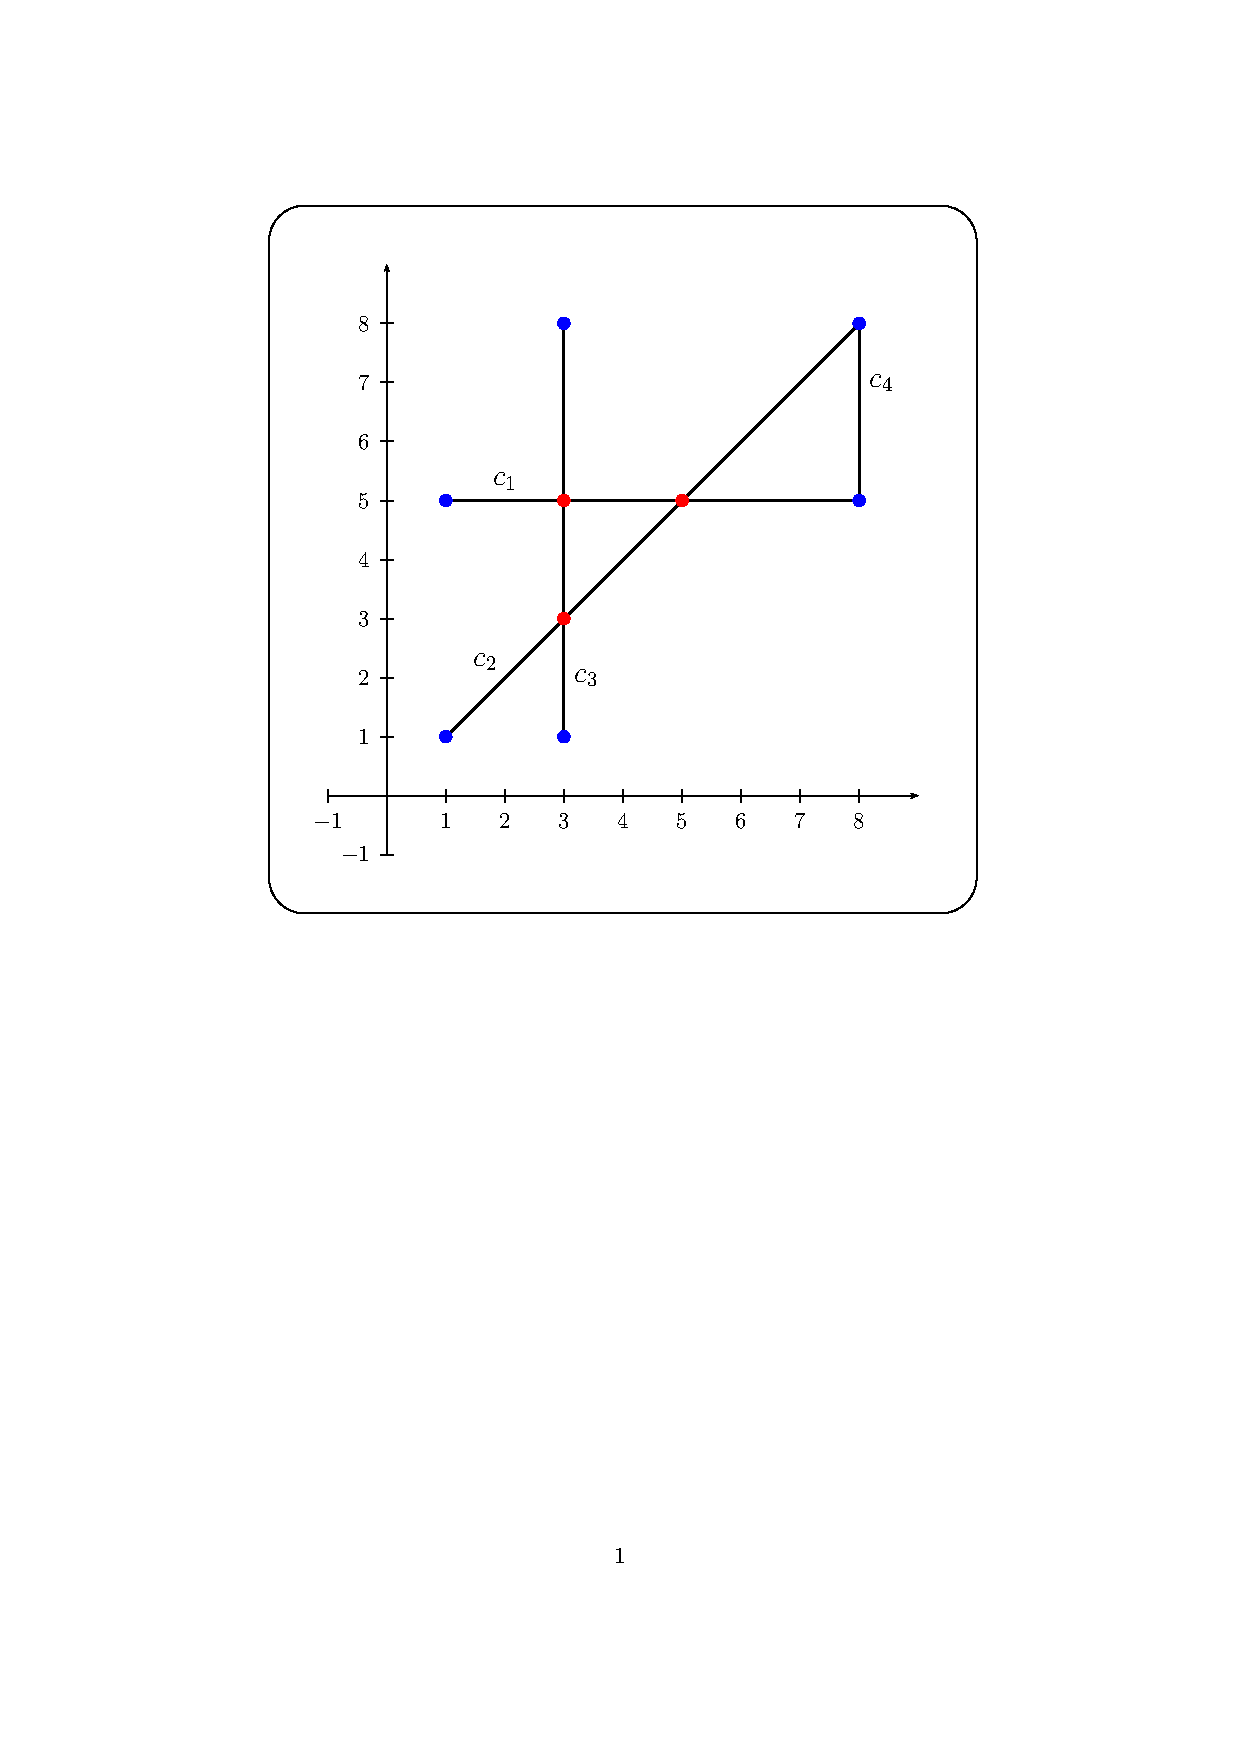
\includegraphics{Sweep_line_2/sl_simple}}
\end{ccTexOnly}

\caption{Four input segments
\label{SL_sec:simple}}

\begin{ccHtmlOnly}
<P>
<center>
  <img src="sl_simple.gif" border=0 alt="Four Input Segments">
</center>
\end{ccHtmlOnly}
\end{figure}

\ccIncludeExampleCode{../examples/Arrangement_2/ex_sweep_line.C}

\section*{Design and Implementation History}
%===========================================
%
The current version of the sweep-line algorithm was written by
Baruch Zukerman, based on previous implementations by Ester Ezra and
Tali Zvi.

